{
\usebackgroundtemplate{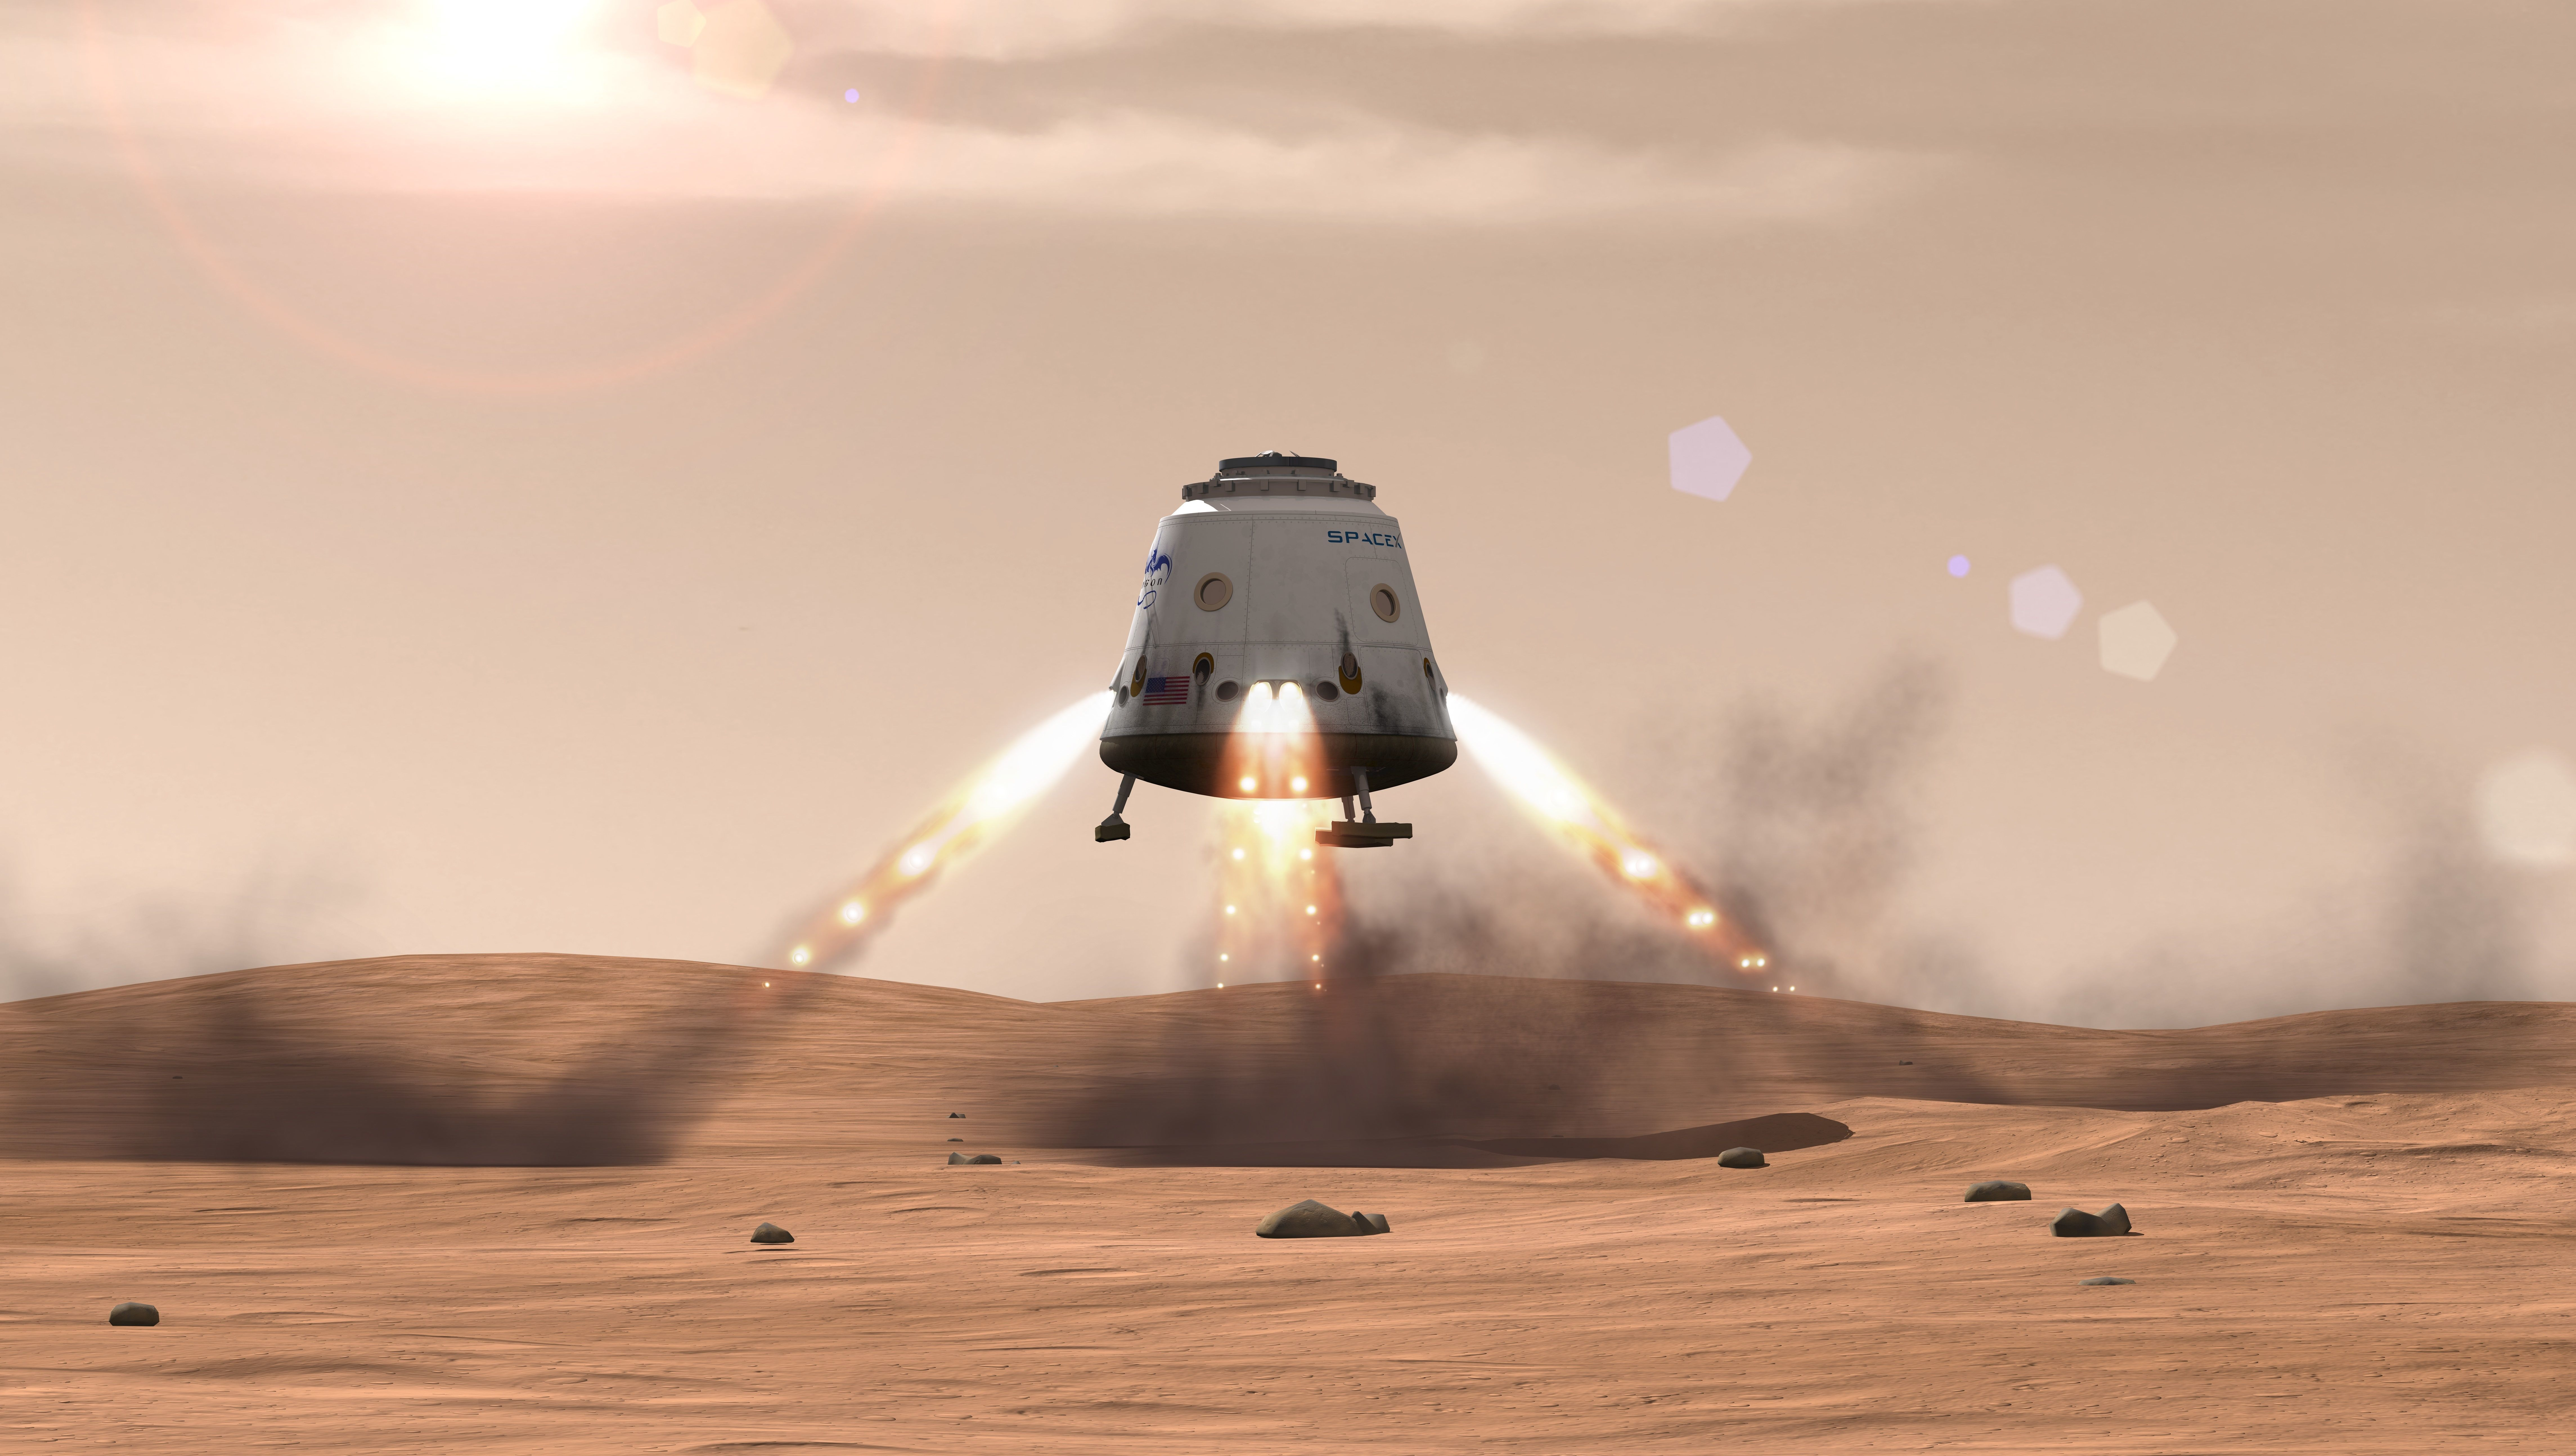
\includegraphics[height=\paperheight, keepaspectratio]{images/landing}}%
\begin{frame}
\end{frame}
\begin{frame}[t]{Landing}
    \begin{block}{Determine entry angle}
        \begin{itemize}
            \item Not to steep, because too much atmosperic drag means we'll burn up
            \item Not to shallow, because we won't slow down quickly enough and skip out of atmosphere
        \end{itemize}
    \end{block}
\end{frame}
\begin{frame}[t]{Landing}
    \begin{block}{Suicide Burn}
        We need to slow down our descent before we hit the ground. At the last possible second we fire all engines at 100\% throttle.
    \end{block}
    \begin{block}{Why?}
        \begin{itemize}
            \item Gravity is accelerating our fall, so decelarating earlier gives gravity more time to accelerate us again
            \item Slowing down quickly saves fuel.
        \end{itemize}
    \end{block}
\end{frame}
}
\begin{frame}[t]{}
    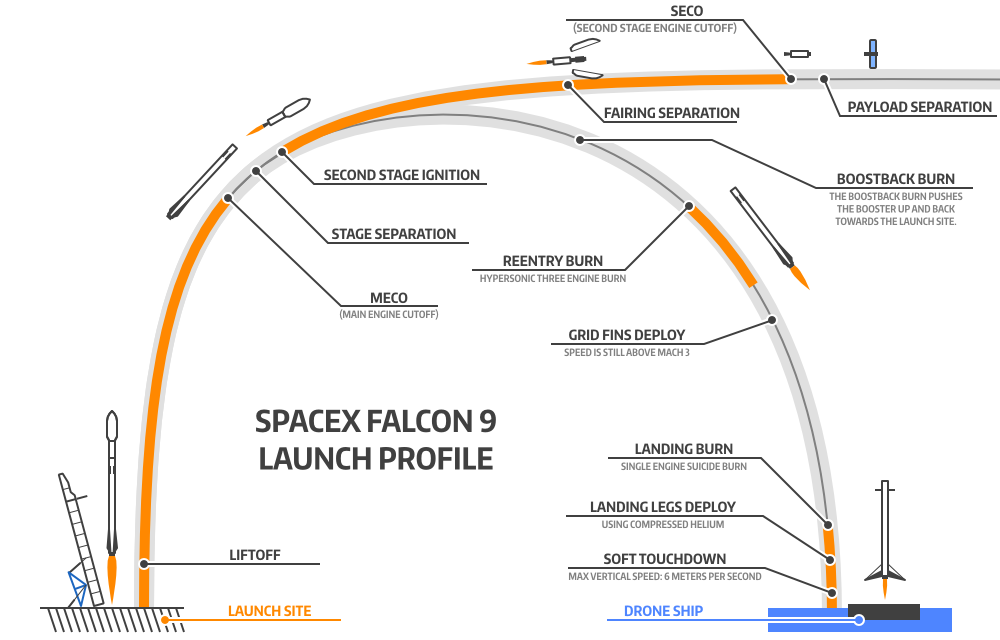
\includegraphics[width=\textwidth]{images/suicideburn}
\end{frame}
{
\usebackgroundtemplate{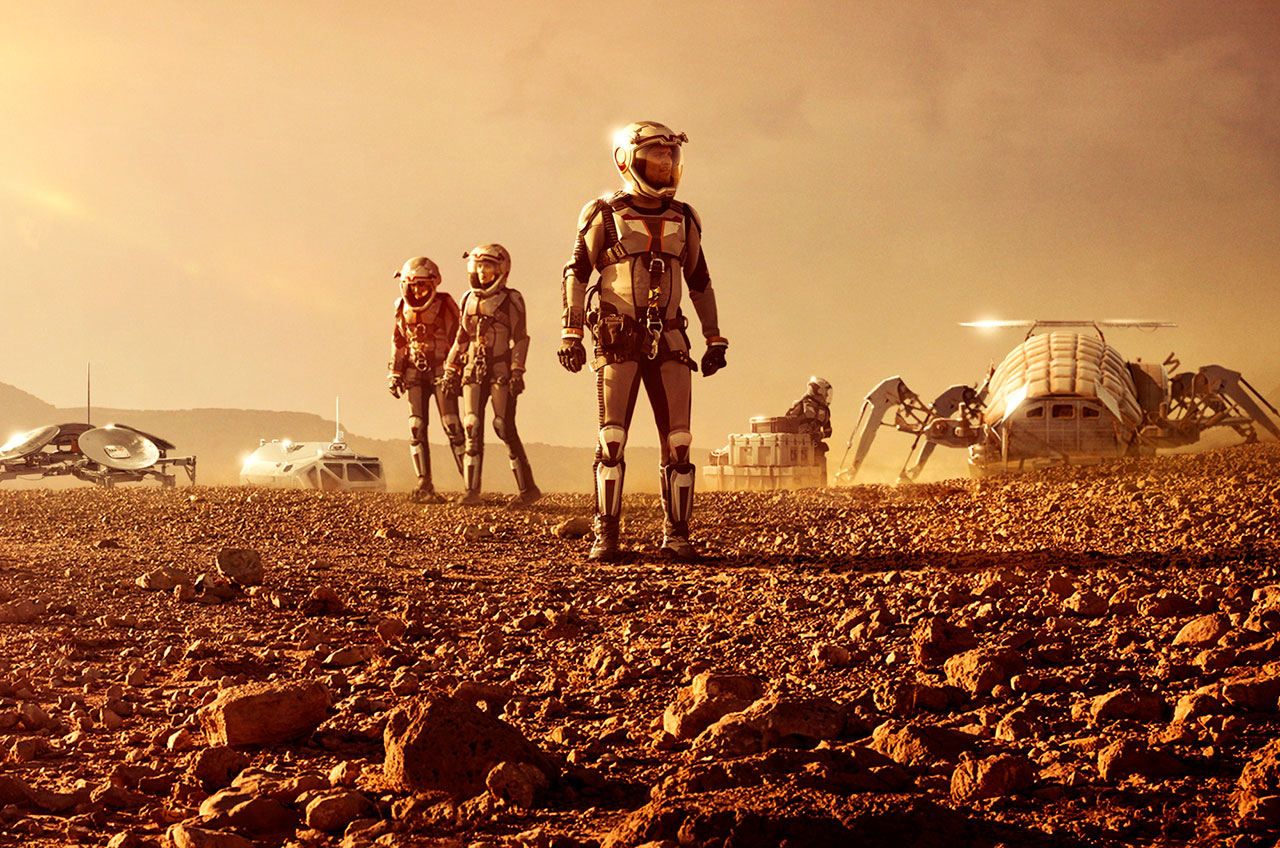
\includegraphics[height=\paperheight, keepaspectratio]{images/landed}}%
\begin{frame}[t]{}
\end{frame}
}
